
We begin by recalling Kolmogorov-Arnold-Moser (KAM) theory, state one of the main KAM theorems, and briefly outline the main points of the theory before delving into its application. We refer the reader to \cite{Knauf_2018} and \cite{Seri_2022} for a more detailed account. We strongly recommend \cite{poschel82} for reference, as it is the version of KAM we use here. What we will see is that for ``small'' values of $b$, our system \eqref{eq:magnetichamiltonian} can be viewed as a perturbation of at least two different Hamiltonian systems, which can explain certain behavior we find. We corroborate our reasoning with many numerical simulations.

\subsection{Summary of KAM theory}
KAM theory is a method for studying perturbations of integrable Hamiltonian systems. Its origins lie in Celestial and Hamiltonian mechanics, where it was used to study the orbits of planets. Hamiltonian mechanics is a strong tool for modeling and studying systems, however it is strongest for conservative systems. Naturally, we find in practice many non-conservative systems, or conservative ones that are too complicated in full, in which case a smaller subsystem is modeled and the rest is viewed as a perturbation. We are interested in the second scenario, we denote by $H^0(q,p)$ an integrable Hamiltonian and by $H^1(q,p,\varepsilon)$ a perturbation. 

Focusing on the integrable case, it is known by the Liouville-Arnold theorem that there exist \textit{action-angle} coordinates so that $H^0:=H^0(p)$ can be expressed in terms of the action variable only. The equations of motion in action-angle coordinates are given by:
\begin{align*}
\dot q = \omega, \qquad \dot p = 0,
\end{align*}
where $\omega = \partial_pH^0(p)$ and $\partial_p H^0:I\to\Omega$ is the so-called \textit{frequency map}. In these action-angle coordinates, the phase space becomes $\mathbb T^n\times I$ where $I\subseteq\mathbb R^n$ and the dynamics of the system are completely expressed as rotations on the torus. Specifically, phase space is foliated into a family of invariant tori $\mathbb T^n\times\{p\}$ for each $p\in I\subseteq \mathbb R^n$. We consider only integrable Hamiltonians with a \textit{non-degenerate} frequency map, that is, $\det\partial_p^2 H^0\neq 0$. Now, KAM deals with Hamiltonians of the form
\begin{align*}
H(q,p) = H^0(p) + \varepsilon H^1(q,p),
\end{align*}
where $1\gg\varepsilon>0$ is considered small, $H^0$ is the integrable part and $H^1$ is the perturbation. We assume that $H$ is $2\pi$-periodic in each component of $q$. What KAM theory ensures is that under the correct conditions, a ``large'' subset $\Omega_{\gamma,\tau}\subseteq\Omega$, $\gamma,\tau>0$ of invariant tori of $H^0(p)$ are preserved, though possibly deformed, under the perturbation $H^1$. The set $\Omega_{\gamma,\tau}$ is given by:
\begin{align}\label{eq:smalldivisorcondition}
\Omega_{\gamma,\tau} = \bigcap_{\substack{k\in\mathbb Z\\ k\neq 0}}\left\{ \omega\in\Omega :
|\omega \cdot k| \ge \gamma|k|^{-\tau}\right\}.
\end{align}
The condition for $\Omega_{\gamma,\tau}$ is called the \textit{small divisor condition}. It can be shown for $\tau>n-1$ that for almost all $x\in\mathbb R^n$ there exists a $\gamma>0$ such that $x\in\Omega_{\gamma,\tau}$, so in particular, we can find $\gamma>0$ so that a point $\omega\in\Omega$ satisfies $\omega\in \Omega_{\gamma,\tau}$. We finally consider the \textit{Cantor} set 
\begin{align*}
\hat\Omega_{\gamma,\tau}= \Omega_{\gamma,\tau}\cap\{\omega\in\Omega: d(\omega,\partial\Omega)\ge\gamma\},
\end{align*}
that is, we remove points in $\Omega_{\gamma,\tau}$ that have distance less than $\gamma$ from the boundary of $\Omega$. It can be shown $\Omega\backslash \bigcup_{\gamma>0}\hat\Omega_{\gamma,\tau}$ is a set of measure zero, so the measure of $\hat\Omega_{\gamma,\tau}$ becomes large for small $\gamma$ ,justifying the term ``large''. We can now give the KAM theorem as stated in \cite{poschel82}.

\begin{theorem}\label{thm:KAM}
Let the integrable Hamiltonian $H^0:\mathbb T^n\times I\to\mathbb R$ be real analytic and non-degenerate, such that the frequency map $\partial_p H^0:I\to\Omega$ is a diffeomorphism and let the perturbed Hamiltonian $H=H^0+\varepsilon H^1$ be of class $C^{\alpha\lambda+\lambda+\tau}$ with $\lambda>\tau+1>n$ and $\alpha>1$. Then there exists a positive $\gamma$-independent $\delta$ such that for $|\varepsilon|<\gamma^2\delta$ with $\gamma$ sufficiently small, there exists a diffeomorphism
\begin{align*}
\mathcal T: \mathbb T^n\times\Omega \to\mathbb T^n\times I,
\end{align*} 
which on $\mathbb T^n\times\hat\Omega_{\gamma,\tau}$ transforms the equations of motion of $H$ into
\begin{align*}
\dot \theta=\omega,\qquad \dot\omega=0.
\end{align*}
The map $\mathcal T$ is of class $C^\alpha$ for non-integer $\alpha$ and close to the inverse of the frequency map; its Jacobian determinant is uniformly bounded from above and below. In addition, if $H$ is of class $C^{\beta\lambda+\lambda+\tau}$ with $\alpha\le\beta\le\infty$, then one can modify $\mathcal T$ outside $\mathbb T^n\times\hat\Omega_{\gamma,\tau}$ so that $\mathcal T$ is of class $C^\beta$ for noninteger $\beta$.
\end{theorem}

So, for $\omega\in\hat\Omega_{\gamma,\tau}$, we parametrize an invariant torus via the map $\theta\mapsto\mathcal T(\theta,\omega)$. There are a few theorems in use now that are titled the \textit{KAM theorem}, and they differ mainly whether they discuss analytic or smooth perturbations. It is easier to find sources discussing the analytic versions, since they provide stronger results about the invariant torii. Having said this, we use the $C^r$ version because it is easier to construct smooth approximations of discontinuous functions as opposed to analytically approximating them. We bring smooth approximations into the mix, since \eqref{eq:magnetichamiltonian} alone is discontinuous.

\subsection{Approximating locally $L^1$ functions}

The Hamiltonian \eqref{eq:magnetichamiltonian} we wish to study is discontinuous, which by itself is not suitable for the KAM theorem. We can, however, smoothly approximate the Hamiltonian by using \textit{mollifiers}. The KAM theorem then can be applied to the smoothed Hamiltonian, which of course means we are not directly studying \eqref{eq:magnetichamiltonian} but instead gaining an intuition for the true behavior.

The \textit{standard mollifier} $\varphi:\mathbb R^n\to\mathbb R$ is the following function:
\begin{align*}
\varphi(x) = \left\{\begin{array}{ll}
c\exp\left(\frac{1}{|x|^2-1}\right), & |x| <1\\
0, & |x|\ge 1,
\end{array}
\right.
\end{align*}
where $c>0$ is a scaling factor chosen so that the integral of $\varphi$ over $\mathbb R^n$ is 1. Also, $\varphi$ is commonly called a \textit{bump} function, since its support is compact. For $\varepsilon>0$, let
\begin{align*}
\varphi_\varepsilon(x) = \frac{1}{\varepsilon^n}\varphi\left(\frac{x}{\varepsilon}\right),
\end{align*} 
this function has the following properties:
\begin{align*}
\varphi_\varepsilon&\in C_c^\infty(\mathbb R^n),\quad
\varphi\ge 0,\\
\int_{\mathbb R^n}&\varphi_\varepsilon =1,\quad
\text{supp}(\varphi_\varepsilon)\subset B_\varepsilon(0)=\{x\in\mathbb R^n:|x|<\varepsilon\},
\end{align*}
that is, the function $\varphi_\varepsilon$ is smooth in $\mathbb R^n$ with compact support, it is positive, its integral is 1, and the support of $\varphi_\varepsilon$ is fully contained in the unit ball of radius $\varepsilon>0$ centered at the origin.
  
Let $f\in L_{\text{loc}}^1(X)$ be a locally integrable function in $X \subseteq\mathbb R^n$. The \textit{mollification} of $f$ is defined as the convolution of $f$ with $\varphi_\varepsilon$, that is, $\varphi_\varepsilon*f:X_\varepsilon\to\mathbb R$ where $X_\varepsilon=\{x\in X: d(x,\partial X)>\varepsilon\}$. Explicitly,
\begin{align*}
f_\varepsilon(x)
  &= \big(\varphi_\varepsilon * f\big)(x)
  = \int_X\varphi_\varepsilon(x-y)f(y)dy\\
  &= \int_{B_\varepsilon(0)}\varphi_\varepsilon(y)f(x-y)dy,\quad x\in X_\varepsilon
\end{align*}

Some properties that the mollification $f_\varepsilon$ has are summarized here:
\begin{theorem}\label{thm:mollification}
Let $f\in L_{\text{loc}}^1(X)$. Then the mollification $f_\varepsilon$ has the following properties:
\begin{enumerate}
\item $f_\varepsilon\in C^\infty(X_\varepsilon)$,
\item $f_\varepsilon\to f$ almost everywhere as $\varepsilon\to0$,
\item if $f$ is continuous on $X$, then $f_\varepsilon\to f$ as $\varepsilon\to0$ uniformly on compact subsebts of $X$,
\item if $1\le p <\infty$ and $f\in L_{\text{loc}}^p(X)$, then $f_\varepsilon\to f$ as $\varepsilon\to 0$ in $L_{\text{loc}}^p(X)$
\end{enumerate}
\end{theorem}
\begin{proof}
The proof of this theorem can be found in Appendix C of \cite{Evans_1998}
\end{proof}

What we gain from \Cref{thm:mollification} is not only a smooth approximation of our discontinuous Hamiltonian but an approximation that can be made arbitrarily precise almost everywhere. Of course, the points which cannot be approximated accurately are concentrated at the boundary of each disk, where the discontinuities lie. Despite this, it is reasonable to assume that for sufficiently small values of $\varepsilon$, the flow of the equations of motion provided by the mollified Hamiltonian approximate the flow of the disconitinuous one very well.


\subsection{Investigating small magnetic field strengths}

In \cref{fig:weakcomparison} we numerically solve the system and observe some interesting relations. Each plot shows 5 trajectories varying $b=10^{-1},\dots,10^{-5}$. In \cref{subfig:weakcomparisonA} and \cref{subfig:weakcomparisonB} the init.~cond.~and params.~are the same $X\approx(0.38,0.81)$ and $V\approx(0,1)$, and $R=1/3$, only the duration of the simulation is longer in \cref{subfig:weakcomparisonB}. In \cref{subfig:weakcomparisonC}, $V$ is the same, $X \approx(0.44,0.65)$ and $R=1/6$. 

First, we see in each figure the trajectory for $b=0.1$ appears as a smear near the origin, this is likely because $b$ is large enough for the deflection in each disk to be significant. We note, however, in later sections we also find circle-like quasiperiodic trajectories for significantly larger values of $b$. The difference here is that these circular arcs seem to be generic, while for larger $b$ the circle-like trajectories are more scarce and each has a smaller region of stability.

For the other values of $b$, we see the trajectories follow a circular arc, and for smaller $b$ the radius of the respective circular arc is larger. In the limit $b\to0$, the trajectories will straighten out, since the magnetic field vanishes. These two observations motivates the use of KAM, specifically, considering \eqref{eq:magnetichamiltonian} as a perturbation of either free motion or of a uniform magnetic field in the plane.


\begin{figure}[!th]
\centering
\hfill
\begin{subfigure}[t]{0.30\textwidth}
\centering
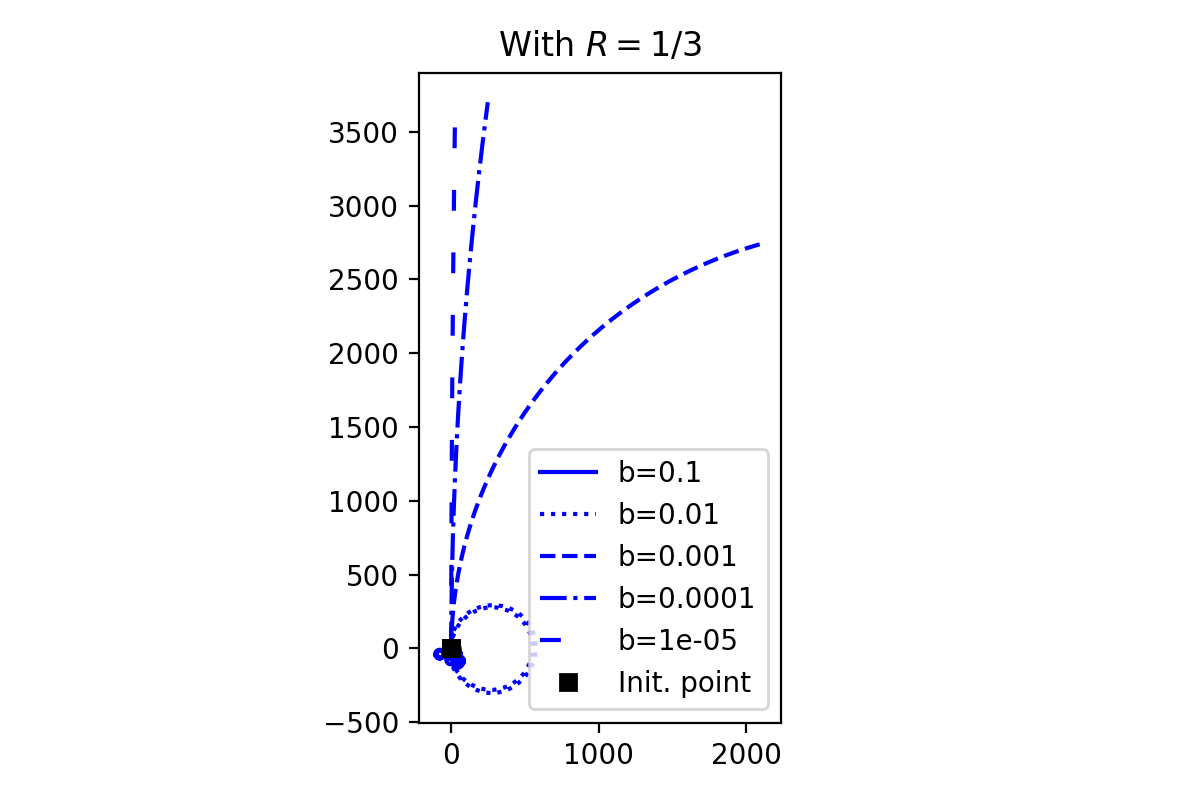
\includegraphics[width=\textwidth, trim={4cm 0cm 4cm 0cm}, clip]{weak_field_comparison_1.png}
\caption{}
\label{subfig:weakcomparisonA}
\end{subfigure}
\hfill
\begin{subfigure}[t]{0.30\textwidth}
\centering
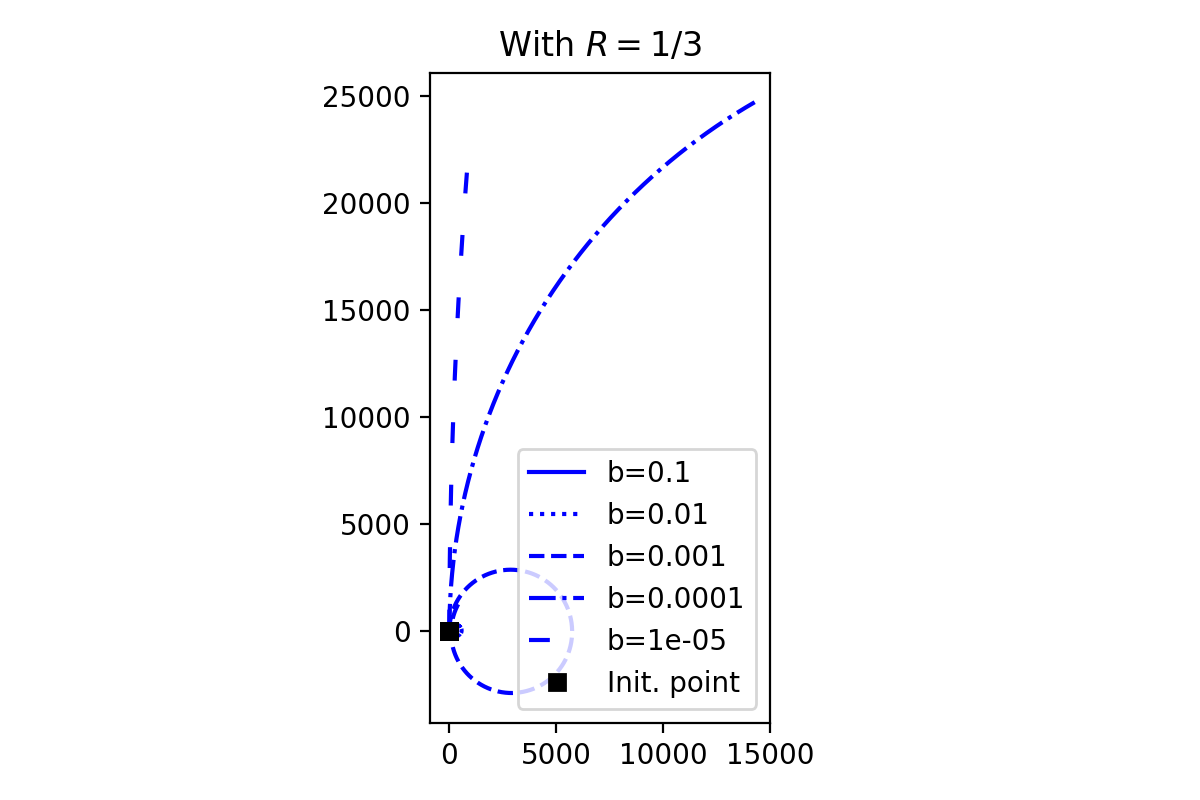
\includegraphics[width=\textwidth, trim={4cm 0 4cm 0}, clip]{weak_field_comparison_2.png}
\caption{}
\label{subfig:weakcomparisonB}
\end{subfigure}
\hfill
\begin{subfigure}[t]{0.30\textwidth}
\centering
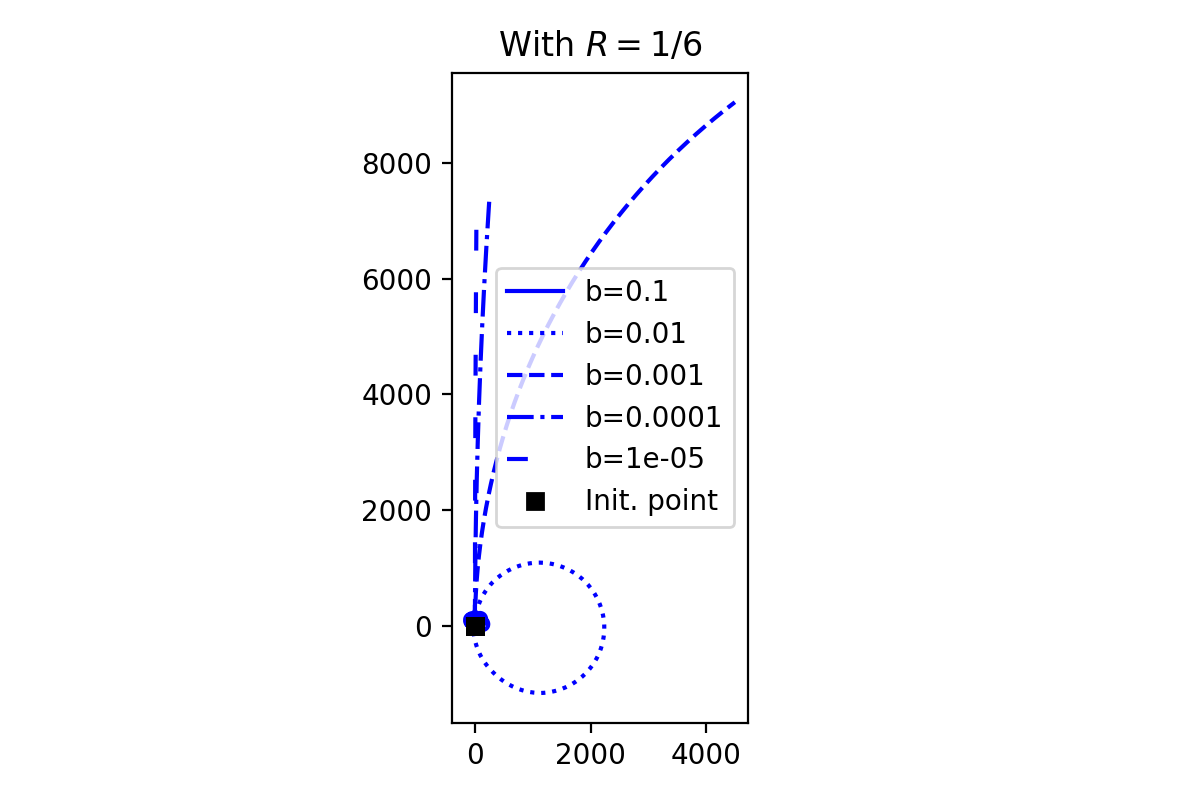
\includegraphics[width=\textwidth, trim={4cm 0 4cm 0}, clip]{weak_field_comparison_3.png}
\caption{}
\label{subfig:weakcomparisonC}
\end{subfigure}
\hfill
\caption{Trajectories for various choices of $R$ and small $b$.}
\label{fig:weakcomparison}
\end{figure}

We note that the free motion perturbation idea seems to be less robust than the uniform field idea. For any small $b>0$, we can expect that after a sufficiently long time $t$ the accumulated deflection is substantial, for example, compare the trajectory for $b=0.0001$ in \cref{subfig:weakcomparisonA} and \cref{subfig:weakcomparisonB}. Having said that, it is not visible in the figure but what appear as circular trajectories in fact do not close either, the displacement is simply very small, but this is precisely what motivated the previous comment: the circles stay circular for longer.